\documentclass[11pt,compress,t,notes=noshow, xcolor=table]{beamer}
\documentclass[11pt,compress,t,notes=noshow, xcolor=table]{beamer}
\usepackage[]{graphicx}\usepackage[]{color}
% maxwidth is the original width if it is less than linewidth
% otherwise use linewidth (to make sure the graphics do not exceed the margin)
\makeatletter
\def\maxwidth{ %
  \ifdim\Gin@nat@width>\linewidth
    \linewidth
  \else
    \Gin@nat@width
  \fi
}
\makeatother

\definecolor{fgcolor}{rgb}{0.345, 0.345, 0.345}
\newcommand{\hlnum}[1]{\textcolor[rgb]{0.686,0.059,0.569}{#1}}%
\newcommand{\hlstr}[1]{\textcolor[rgb]{0.192,0.494,0.8}{#1}}%
\newcommand{\hlcom}[1]{\textcolor[rgb]{0.678,0.584,0.686}{\textit{#1}}}%
\newcommand{\hlopt}[1]{\textcolor[rgb]{0,0,0}{#1}}%
\newcommand{\hlstd}[1]{\textcolor[rgb]{0.345,0.345,0.345}{#1}}%
\newcommand{\hlkwa}[1]{\textcolor[rgb]{0.161,0.373,0.58}{\textbf{#1}}}%
\newcommand{\hlkwb}[1]{\textcolor[rgb]{0.69,0.353,0.396}{#1}}%
\newcommand{\hlkwc}[1]{\textcolor[rgb]{0.333,0.667,0.333}{#1}}%
\newcommand{\hlkwd}[1]{\textcolor[rgb]{0.737,0.353,0.396}{\textbf{#1}}}%
\let\hlipl\hlkwb

\usepackage{framed}
\makeatletter
\newenvironment{kframe}{%
 \def\at@end@of@kframe{}%
 \ifinner\ifhmode%
  \def\at@end@of@kframe{\end{minipage}}%
  \begin{minipage}{\columnwidth}%
 \fi\fi%
 \def\FrameCommand##1{\hskip\@totalleftmargin \hskip-\fboxsep
 \colorbox{shadecolor}{##1}\hskip-\fboxsep
     % There is no \\@totalrightmargin, so:
     \hskip-\linewidth \hskip-\@totalleftmargin \hskip\columnwidth}%
 \MakeFramed {\advance\hsize-\width
   \@totalleftmargin\z@ \linewidth\hsize
   \@setminipage}}%
 {\par\unskip\endMakeFramed%
 \at@end@of@kframe}
\makeatother

\definecolor{shadecolor}{rgb}{.97, .97, .97}
\definecolor{messagecolor}{rgb}{0, 0, 0}
\definecolor{warningcolor}{rgb}{1, 0, 1}
\definecolor{errorcolor}{rgb}{1, 0, 0}
\newenvironment{knitrout}{}{} % an empty environment to be redefined in TeX

\usepackage{alltt}
\newcommand{\SweaveOpts}[1]{}  % do not interfere with LaTeX
\newcommand{\SweaveInput}[1]{} % because they are not real TeX commands
\newcommand{\Sexpr}[1]{}       % will only be parsed by R
\newcommand{\xmark}{\ding{55}}%


\usepackage[english]{babel}
\usepackage[utf8]{inputenc}

\usepackage{dsfont}
\usepackage{verbatim}
\usepackage{amsmath}
\usepackage{amsfonts}
\usepackage{amssymb}
\usepackage{bm}
\usepackage{csquotes}
\usepackage{multirow}
\usepackage{longtable}
\usepackage{booktabs}
\usepackage{enumerate}
\usepackage[absolute,overlay]{textpos}
\usepackage{psfrag}
\usepackage{algorithm}
\usepackage{algpseudocode}
\usepackage{eqnarray}
\usepackage{arydshln}
\usepackage{tabularx}
\usepackage{placeins}
\usepackage{tikz}
\usepackage{setspace}
\usepackage{colortbl}
\usepackage{mathtools}
\usepackage{wrapfig}
\usepackage{bm}
\usepackage{amsmath}
\usepackage{pifont}

\usetikzlibrary{shapes,arrows,automata,positioning,calc,chains,trees, shadows}
\tikzset{
  %Define standard arrow tip
  >=stealth',
  %Define style for boxes
  punkt/.style={
    rectangle,
    rounded corners,
    draw=black, very thick,
    text width=6.5em,
    minimum height=2em,
    text centered},
  % Define arrow style
  pil/.style={
    ->,
    thick,
    shorten <=2pt,
    shorten >=2pt,}
}

\usepackage{subfig}

% Defines macros and environments
\usepackage{../../style/lmu-lecture}


\let\code=\texttt
\let\proglang=\textsf

\setkeys{Gin}{width=0.9\textwidth}

\setbeamertemplate{frametitle}{\expandafter\uppercase\expandafter\insertframetitle}

% This file is included in slides and exercises

% Rarely used fontstyle for R packages, used only in 
% - forests/slides-forests-benchmark.tex
% - exercises/single-exercises/methods_l_1.Rnw
% - slides/cart/attic/slides_extra_trees.Rnw
\newcommand{\pkg}[1]{{\fontseries{b}\selectfont #1}}

% Spacing helpers, used often (mostly in exercises for \dlz)
\newcommand{\lz}{\vspace{0.5cm}} % vertical space (used often in slides)
\newcommand{\dlz}{\vspace{1cm}}  % double vertical space (used often in exercises, never in slides)
\newcommand{\oneliner}[1] % Oneliner for important statements, used e.g. in iml, algods
{\begin{block}{}\begin{center}\begin{Large}#1\end{Large}\end{center}\end{block}}

% Don't know if this is used or needed, remove?
% textcolor that works in mathmode
% https://tex.stackexchange.com/a/261480
% Used e.g. in forests/slides-forests-bagging.tex
% [...] \textcolor{blue}{\tfrac{1}{M}\sum^M_{m} [...]
% \makeatletter
% \renewcommand*{\@textcolor}[3]{%
%   \protect\leavevmode
%   \begingroup
%     \color#1{#2}#3%
%   \endgroup
% }
% \makeatother






% latex-math includes as needed
% dependencies: amsmath, amssymb, dsfont
% math spaces
\ifdefined\N
\renewcommand{\N}{\mathds{N}} % N, naturals
\else \newcommand{\N}{\mathds{N}} \fi
\newcommand{\Z}{\mathds{Z}} % Z, integers
\newcommand{\Q}{\mathds{Q}} % Q, rationals
\newcommand{\R}{\mathds{R}} % R, reals
\ifdefined\C
\renewcommand{\C}{\mathds{C}} % C, complex
\else \newcommand{\C}{\mathds{C}} \fi
\newcommand{\continuous}{\mathcal{C}} % C, space of continuous functions
\newcommand{\M}{\mathcal{M}} % machine numbers
\newcommand{\epsm}{\epsilon_m} % maximum error

% counting / finite sets
\newcommand{\setzo}{\{0, 1\}} % set 0, 1
\newcommand{\setmp}{\{-1, +1\}} % set -1, 1
\newcommand{\unitint}{[0, 1]} % unit interval

% basic math stuff
\newcommand{\xt}{\tilde x} % x tilde
\newcommand{\argmin}{\mathop{\mathrm{arg\,min}}} % argmin
\newcommand{\argmax}{\mathop{\mathrm{arg\,max}}} % argmax
\newcommand{\argminlim}{\argmin\limits} % argmin with limits
\newcommand{\argmaxlim}{\argmax\limits} % argmax with limits
\newcommand{\sign}{\operatorname{sign}} % sign, signum
\newcommand{\I}{\mathbb{I}} % I, indicator
\newcommand{\order}{\mathcal{O}} % O, order
\newcommand{\bigO}{\mathcal{O}} % Big-O Landau
\newcommand{\littleo}{{o}} % Little-o Landau
\newcommand{\pd}[2]{\frac{\partial{#1}}{\partial #2}} % partial derivative
\newcommand{\floorlr}[1]{\left\lfloor #1 \right\rfloor} % floor
\newcommand{\ceillr}[1]{\left\lceil #1 \right\rceil} % ceiling
\newcommand{\indep}{\perp \!\!\! \perp} % independence symbol

% sums and products
\newcommand{\sumin}{\sum\limits_{i=1}^n} % summation from i=1 to n
\newcommand{\sumim}{\sum\limits_{i=1}^m} % summation from i=1 to m
\newcommand{\sumjn}{\sum\limits_{j=1}^n} % summation from j=1 to p
\newcommand{\sumjp}{\sum\limits_{j=1}^p} % summation from j=1 to p
\newcommand{\sumik}{\sum\limits_{i=1}^k} % summation from i=1 to k
\newcommand{\sumkg}{\sum\limits_{k=1}^g} % summation from k=1 to g
\newcommand{\sumjg}{\sum\limits_{j=1}^g} % summation from j=1 to g
\newcommand{\summM}{\sum\limits_{m=1}^M} % summation from m=1 to M
\newcommand{\meanin}{\frac{1}{n} \sum\limits_{i=1}^n} % mean from i=1 to n
\newcommand{\meanim}{\frac{1}{m} \sum\limits_{i=1}^m} % mean from i=1 to n
\newcommand{\meankg}{\frac{1}{g} \sum\limits_{k=1}^g} % mean from k=1 to g
\newcommand{\meanmM}{\frac{1}{M} \sum\limits_{m=1}^M} % mean from m=1 to M
\newcommand{\prodin}{\prod\limits_{i=1}^n} % product from i=1 to n
\newcommand{\prodkg}{\prod\limits_{k=1}^g} % product from k=1 to g
\newcommand{\prodjp}{\prod\limits_{j=1}^p} % product from j=1 to p

% linear algebra
\newcommand{\one}{\bm{1}} % 1, unitvector
\newcommand{\zero}{\mathbf{0}} % 0-vector
\newcommand{\id}{\bm{I}} % I, identity
\newcommand{\diag}{\operatorname{diag}} % diag, diagonal
\newcommand{\trace}{\operatorname{tr}} % tr, trace
\newcommand{\spn}{\operatorname{span}} % span
\newcommand{\scp}[2]{\left\langle #1, #2 \right\rangle} % <.,.>, scalarproduct
\newcommand{\mat}[1]{\begin{pmatrix} #1 \end{pmatrix}} % short pmatrix command
\newcommand{\Amat}{\mathbf{A}} % matrix A
\newcommand{\Deltab}{\mathbf{\Delta}} % error term for vectors

% basic probability + stats
\renewcommand{\P}{\mathds{P}} % P, probability
\newcommand{\E}{\mathds{E}} % E, expectation
\newcommand{\var}{\mathsf{Var}} % Var, variance
\newcommand{\cov}{\mathsf{Cov}} % Cov, covariance
\newcommand{\corr}{\mathsf{Corr}} % Corr, correlation
\newcommand{\normal}{\mathcal{N}} % N of the normal distribution
\newcommand{\iid}{\overset{i.i.d}{\sim}} % dist with i.i.d superscript
\newcommand{\distas}[1]{\overset{#1}{\sim}} % ... is distributed as ...

% machine learning
\newcommand{\Xspace}{\mathcal{X}} % X, input space
\newcommand{\Yspace}{\mathcal{Y}} % Y, output space
\newcommand{\Zspace}{\mathcal{Z}} % Z, space of sampled datapoints
\newcommand{\nset}{\{1, \ldots, n\}} % set from 1 to n
\newcommand{\pset}{\{1, \ldots, p\}} % set from 1 to p
\newcommand{\gset}{\{1, \ldots, g\}} % set from 1 to g
\newcommand{\Pxy}{\mathbb{P}_{xy}} % P_xy
\newcommand{\Exy}{\mathbb{E}_{xy}} % E_xy: Expectation over random variables xy
\newcommand{\xv}{\mathbf{x}} % vector x (bold)
\newcommand{\xtil}{\tilde{\mathbf{x}}} % vector x-tilde (bold)
\newcommand{\yv}{\mathbf{y}} % vector y (bold)
\newcommand{\xy}{(\xv, y)} % observation (x, y)
\newcommand{\xvec}{\left(x_1, \ldots, x_p\right)^\top} % (x1, ..., xp)
\newcommand{\Xmat}{\mathbf{X}} % Design matrix
\newcommand{\allDatasets}{\mathds{D}} % The set of all datasets
\newcommand{\allDatasetsn}{\mathds{D}_n}  % The set of all datasets of size n
\newcommand{\D}{\mathcal{D}} % D, data
\newcommand{\Dn}{\D_n} % D_n, data of size n
\newcommand{\Dtrain}{\mathcal{D}_{\text{train}}} % D_train, training set
\newcommand{\Dtest}{\mathcal{D}_{\text{test}}} % D_test, test set
\newcommand{\xyi}[1][i]{\left(\xv^{(#1)}, y^{(#1)}\right)} % (x^i, y^i), i-th observation
\newcommand{\Dset}{\left( \xyi[1], \ldots, \xyi[n]\right)} % {(x1,y1)), ..., (xn,yn)}, data
\newcommand{\defAllDatasetsn}{(\Xspace \times \Yspace)^n} % Def. of the set of all datasets of size n
\newcommand{\defAllDatasets}{\bigcup_{n \in \N}(\Xspace \times \Yspace)^n} % Def. of the set of all datasets
\newcommand{\xdat}{\left\{ \xv^{(1)}, \ldots, \xv^{(n)}\right\}} % {x1, ..., xn}, input data
\newcommand{\ydat}{\left\{ \yv^{(1)}, \ldots, \yv^{(n)}\right\}} % {y1, ..., yn}, input data
\newcommand{\yvec}{\left(y^{(1)}, \hdots, y^{(n)}\right)^\top} % (y1, ..., yn), vector of outcomes
\newcommand{\greekxi}{\xi} % Greek letter xi
\renewcommand{\xi}[1][i]{\xv^{(#1)}} % x^i, i-th observed value of x
\newcommand{\yi}[1][i]{y^{(#1)}} % y^i, i-th observed value of y
\newcommand{\xivec}{\left(x^{(i)}_1, \ldots, x^{(i)}_p\right)^\top} % (x1^i, ..., xp^i), i-th observation vector
\newcommand{\xj}{\xv_j} % x_j, j-th feature
\newcommand{\xjvec}{\left(x^{(1)}_j, \ldots, x^{(n)}_j\right)^\top} % (x^1_j, ..., x^n_j), j-th feature vector
\newcommand{\phiv}{\mathbf{\phi}} % Basis transformation function phi
\newcommand{\phixi}{\mathbf{\phi}^{(i)}} % Basis transformation of xi: phi^i := phi(xi)

%%%%%% ml - models general
\newcommand{\lamv}{\bm{\lambda}} % lambda vector, hyperconfiguration vector
\newcommand{\Lam}{\bm{\Lambda}}	 % Lambda, space of all hpos
% Inducer / Inducing algorithm
\newcommand{\preimageInducer}{\left(\defAllDatasets\right)\times\Lam} % Set of all datasets times the hyperparameter space
\newcommand{\preimageInducerShort}{\allDatasets\times\Lam} % Set of all datasets times the hyperparameter space
% Inducer / Inducing algorithm
\newcommand{\ind}{\mathcal{I}} % Inducer, inducing algorithm, learning algorithm

% continuous prediction function f
\newcommand{\ftrue}{f_{\text{true}}}  % True underlying function (if a statistical model is assumed)
\newcommand{\ftruex}{\ftrue(\xv)} % True underlying function (if a statistical model is assumed)
\newcommand{\fx}{f(\xv)} % f(x), continuous prediction function
\newcommand{\fdomains}{f: \Xspace \rightarrow \R^g} % f with domain and co-domain
\newcommand{\Hspace}{\mathcal{H}} % hypothesis space where f is from
\newcommand{\fbayes}{f^{\ast}} % Bayes-optimal model
\newcommand{\fxbayes}{f^{\ast}(\xv)} % Bayes-optimal model
\newcommand{\fkx}[1][k]{f_{#1}(\xv)} % f_j(x), discriminant component function
\newcommand{\fh}{\hat{f}} % f hat, estimated prediction function
\newcommand{\fxh}{\fh(\xv)} % fhat(x)
\newcommand{\fxt}{f(\xv ~|~ \thetav)} % f(x | theta)
\newcommand{\fxi}{f\left(\xv^{(i)}\right)} % f(x^(i))
\newcommand{\fxih}{\hat{f}\left(\xv^{(i)}\right)} % f(x^(i))
\newcommand{\fxit}{f\left(\xv^{(i)} ~|~ \thetav\right)} % f(x^(i) | theta)
\newcommand{\fhD}{\fh_{\D}} % fhat_D, estimate of f based on D
\newcommand{\fhDtrain}{\fh_{\Dtrain}} % fhat_Dtrain, estimate of f based on D
\newcommand{\fhDnlam}{\fh_{\Dn, \lamv}} %model learned on Dn with hp lambda
\newcommand{\fhDlam}{\fh_{\D, \lamv}} %model learned on D with hp lambda
\newcommand{\fhDnlams}{\fh_{\Dn, \lamv^\ast}} %model learned on Dn with optimal hp lambda
\newcommand{\fhDlams}{\fh_{\D, \lamv^\ast}} %model learned on D with optimal hp lambda

% discrete prediction function h
\newcommand{\hx}{h(\xv)} % h(x), discrete prediction function
\newcommand{\hh}{\hat{h}} % h hat
\newcommand{\hxh}{\hat{h}(\xv)} % hhat(x)
\newcommand{\hxt}{h(\xv | \thetav)} % h(x | theta)
\newcommand{\hxi}{h\left(\xi\right)} % h(x^(i))
\newcommand{\hxit}{h\left(\xi ~|~ \thetav\right)} % h(x^(i) | theta)
\newcommand{\hbayes}{h^{\ast}} % Bayes-optimal classification model
\newcommand{\hxbayes}{h^{\ast}(\xv)} % Bayes-optimal classification model

% yhat
\newcommand{\yh}{\hat{y}} % yhat for prediction of target
\newcommand{\yih}{\hat{y}^{(i)}} % yhat^(i) for prediction of ith targiet
\newcommand{\resi}{\yi- \yih}

% theta
\newcommand{\thetah}{\hat{\theta}} % theta hat
\newcommand{\thetav}{\bm{\theta}} % theta vector
\newcommand{\thetavh}{\bm{\hat\theta}} % theta vector hat
\newcommand{\thetat}[1][t]{\thetav^{[#1]}} % theta^[t] in optimization
\newcommand{\thetatn}[1][t]{\thetav^{[#1 +1]}} % theta^[t+1] in optimization
\newcommand{\thetahDnlam}{\thetavh_{\Dn, \lamv}} %theta learned on Dn with hp lambda
\newcommand{\thetahDlam}{\thetavh_{\D, \lamv}} %theta learned on D with hp lambda
\newcommand{\mint}{\min_{\thetav \in \Theta}} % min problem theta
\newcommand{\argmint}{\argmin_{\thetav \in \Theta}} % argmin theta

% densities + probabilities
% pdf of x
\newcommand{\pdf}{p} % p
\newcommand{\pdfx}{p(\xv)} % p(x)
\newcommand{\pixt}{\pi(\xv~|~ \thetav)} % pi(x|theta), pdf of x given theta
\newcommand{\pixit}[1][i]{\pi\left(\xi[#1] ~|~ \thetav\right)} % pi(x^i|theta), pdf of x given theta
\newcommand{\pixii}[1][i]{\pi\left(\xi[#1]\right)} % pi(x^i), pdf of i-th x

% pdf of (x, y)
\newcommand{\pdfxy}{p(\xv,y)} % p(x, y)
\newcommand{\pdfxyt}{p(\xv, y ~|~ \thetav)} % p(x, y | theta)
\newcommand{\pdfxyit}{p\left(\xi, \yi ~|~ \thetav\right)} % p(x^(i), y^(i) | theta)

% pdf of x given y
\newcommand{\pdfxyk}[1][k]{p(\xv | y= #1)} % p(x | y = k)
\newcommand{\lpdfxyk}[1][k]{\log p(\xv | y= #1)} % log p(x | y = k)
\newcommand{\pdfxiyk}[1][k]{p\left(\xi | y= #1 \right)} % p(x^i | y = k)

% prior probabilities
\newcommand{\pik}[1][k]{\pi_{#1}} % pi_k, prior
\newcommand{\lpik}[1][k]{\log \pi_{#1}} % log pi_k, log of the prior
\newcommand{\pit}{\pi(\thetav)} % Prior probability of parameter theta

% posterior probabilities
\newcommand{\post}{\P(y = 1 ~|~ \xv)} % P(y = 1 | x), post. prob for y=1
\newcommand{\postk}[1][k]{\P(y = #1 ~|~ \xv)} % P(y = k | y), post. prob for y=k
\newcommand{\pidomains}{\pi: \Xspace \rightarrow \unitint} % pi with domain and co-domain
\newcommand{\pibayes}{\pi^{\ast}} % Bayes-optimal classification model
\newcommand{\pixbayes}{\pi^{\ast}(\xv)} % Bayes-optimal classification model
\newcommand{\pix}{\pi(\xv)} % pi(x), P(y = 1 | x)
\newcommand{\piv}{\bm{\pi}} % pi, bold, as vector
\newcommand{\pikx}[1][k]{\pi_{#1}(\xv)} % pi_k(x), P(y = k | x)
\newcommand{\pikxt}[1][k]{\pi_{#1}(\xv ~|~ \thetav)} % pi_k(x | theta), P(y = k | x, theta)
\newcommand{\pixh}{\hat \pi(\xv)} % pi(x) hat, P(y = 1 | x) hat
\newcommand{\pikxh}[1][k]{\hat \pi_{#1}(\xv)} % pi_k(x) hat, P(y = k | x) hat
\newcommand{\pixih}{\hat \pi(\xi)} % pi(x^(i)) with hat
\newcommand{\pikxih}[1][k]{\hat \pi_{#1}(\xi)} % pi_k(x^(i)) with hat
\newcommand{\pdfygxt}{p(y ~|~\xv, \thetav)} % p(y | x, theta)
\newcommand{\pdfyigxit}{p\left(\yi ~|~\xi, \thetav\right)} % p(y^i |x^i, theta)
\newcommand{\lpdfygxt}{\log \pdfygxt } % log p(y | x, theta)
\newcommand{\lpdfyigxit}{\log \pdfyigxit} % log p(y^i |x^i, theta)

% probababilistic
\newcommand{\bayesrulek}[1][k]{\frac{\P(\xv | y= #1) \P(y= #1)}{\P(\xv)}} % Bayes rule
\newcommand{\muk}{\bm{\mu_k}} % mean vector of class-k Gaussian (discr analysis)

% residual and margin
\newcommand{\eps}{\epsilon} % residual, stochastic
\newcommand{\epsv}{\bm{\epsilon}} % residual, stochastic, as vector
\newcommand{\epsi}{\epsilon^{(i)}} % epsilon^i, residual, stochastic
\newcommand{\epsh}{\hat{\epsilon}} % residual, estimated
\newcommand{\epsvh}{\hat{\epsv}} % residual, estimated, vector
\newcommand{\yf}{y \fx} % y f(x), margin
\newcommand{\yfi}{\yi \fxi} % y^i f(x^i), margin
\newcommand{\Sigmah}{\hat \Sigma} % estimated covariance matrix
\newcommand{\Sigmahj}{\hat \Sigma_j} % estimated covariance matrix for the j-th class

% ml - loss, risk, likelihood
\newcommand{\Lyf}{L\left(y, f\right)} % L(y, f), loss function
\newcommand{\Lypi}{L\left(y, \pi\right)} % L(y, pi), loss function
\newcommand{\Lxy}{L\left(y, \fx\right)} % L(y, f(x)), loss function
\newcommand{\Lxyi}{L\left(\yi, \fxi\right)} % loss of observation
\newcommand{\Lxyt}{L\left(y, \fxt\right)} % loss with f parameterized
\newcommand{\Lxyit}{L\left(\yi, \fxit\right)} % loss of observation with f parameterized
\newcommand{\Lxym}{L\left(\yi, f\left(\bm{\tilde{x}}^{(i)} ~|~ \thetav\right)\right)} % loss of observation with f parameterized
\newcommand{\Lpixy}{L\left(y, \pix\right)} % loss in classification
\newcommand{\Lpiy}{L\left(y, \pi\right)} % loss in classification
\newcommand{\Lpiv}{L\left(y, \piv\right)} % loss in classification
\newcommand{\Lpixyi}{L\left(\yi, \pixii\right)} % loss of observation in classification
\newcommand{\Lpixyt}{L\left(y, \pixt\right)} % loss with pi parameterized
\newcommand{\Lpixyit}{L\left(\yi, \pixit\right)} % loss of observation with pi parameterized
\newcommand{\Lhy}{L\left(y, h\right)} % L(y, h), loss function on discrete classes
\newcommand{\Lhxy}{L\left(y, \hx\right)} % L(y, h(x)), loss function on discrete classes
\newcommand{\Lr}{L\left(r\right)} % L(r), loss defined on residual (reg) / margin (classif)
\newcommand{\lone}{|y - \fx|} % L1 loss
\newcommand{\ltwo}{\left(y - \fx\right)^2} % L2 loss
\newcommand{\lbernoullimp}{\ln(1 + \exp(-y \cdot \fx))} % Bernoulli loss for -1, +1 encoding
\newcommand{\lbernoullizo}{- y \cdot \fx + \log(1 + \exp(\fx))} % Bernoulli loss for 0, 1 encoding
\newcommand{\lcrossent}{- y \log \left(\pix\right) - (1 - y) \log \left(1 - \pix\right)} % cross-entropy loss
\newcommand{\lbrier}{\left(\pix - y \right)^2} % Brier score
\newcommand{\risk}{\mathcal{R}} % R, risk
\newcommand{\riskbayes}{\mathcal{R}^\ast}
\newcommand{\riskf}{\risk(f)} % R(f), risk
\newcommand{\riskdef}{\E_{y|\xv}\left(\Lxy \right)} % risk def (expected loss)
\newcommand{\riskt}{\mathcal{R}(\thetav)} % R(theta), risk
\newcommand{\riske}{\mathcal{R}_{\text{emp}}} % R_emp, empirical risk w/o factor 1 / n
\newcommand{\riskeb}{\bar{\mathcal{R}}_{\text{emp}}} % R_emp, empirical risk w/ factor 1 / n
\newcommand{\riskef}{\riske(f)} % R_emp(f)
\newcommand{\risket}{\mathcal{R}_{\text{emp}}(\thetav)} % R_emp(theta)
\newcommand{\riskr}{\mathcal{R}_{\text{reg}}} % R_reg, regularized risk
\newcommand{\riskrt}{\mathcal{R}_{\text{reg}}(\thetav)} % R_reg(theta)
\newcommand{\riskrf}{\riskr(f)} % R_reg(f)
\newcommand{\riskrth}{\hat{\mathcal{R}}_{\text{reg}}(\thetav)} % hat R_reg(theta)
\newcommand{\risketh}{\hat{\mathcal{R}}_{\text{emp}}(\thetav)} % hat R_emp(theta)
\newcommand{\LL}{\mathcal{L}} % L, likelihood
\newcommand{\LLt}{\mathcal{L}(\thetav)} % L(theta), likelihood
\newcommand{\LLtx}{\mathcal{L}(\thetav | \xv)} % L(theta|x), likelihood
\newcommand{\logl}{\ell} % l, log-likelihood
\newcommand{\loglt}{\logl(\thetav)} % l(theta), log-likelihood
\newcommand{\logltx}{\logl(\thetav | \xv)} % l(theta|x), log-likelihood
\newcommand{\errtrain}{\text{err}_{\text{train}}} % training error
\newcommand{\errtest}{\text{err}_{\text{test}}} % test error
\newcommand{\errexp}{\overline{\text{err}_{\text{test}}}} % avg training error

% lm
\newcommand{\thx}{\thetav^\top \xv} % linear model
\newcommand{\olsest}{(\Xmat^\top \Xmat)^{-1} \Xmat^\top \yv} % OLS estimator in LM


% Lecture title always has to be there
\title{Algorithms and Data Structures}

\begin{document}

\titlemeta{% Chunk title (example: CART, Forests, Boosting, ...), can be empty
Matrix Decomposition
}{% Lecture title
QR Decomposition
}{% Relative path to title page image: Can be empty but must not start with slides/
}{% Learning goals, wrapped inside itemize environment
  \item Misconceptions
  \item Alternative notations
  \item Complexity vs. empirical runtime
}
%\lecture{CIM1 Statistical Computing}

\begin{vbframe}{QR decomposition}

% Als Alternative zu Cholesky wird mitunter die QR-Zerlegung angewandt.

Given $\Amat \in \R^{n \times n}$. We decompose $\Amat$ into the product of an orthogonal matrix $\bm{Q}\in \R^{n \times n}$ and an upper triangular matrix $\bm{R} \in \R^{n \times n}$

$$
\Amat = \bm{QR} \quad \mbox{with} \quad \bm{Q}^\top\bm{Q} = \bm{I},
$$

The columns of the matrix $\bm{Q} = (\bm{q}_1, \ldots, \bm{q}_n)$ form an orthonormal basis for the column space of the matrix $\Amat$ and

$$
\bm{R} = \mat{
\langle \bm{q_1}, \bm{a_1} \rangle & \langle \bm{q_1}, \bm{a_2} \rangle & \langle \bm{q_1}, \bm{a_3} \rangle & \cdots \\
0                                  & \langle \bm{q_2}, \bm{a_2} \rangle & \langle \bm{q_2}, \bm{a_3} \rangle & \cdots \\
0                                  & 0                                  & \langle \bm{q_3}, \bm{a_3} \rangle & \cdots \\
\vdots                             & \vdots                             & \vdots                             & \ddots \\}
$$

The orthonormal basis for $\Amat$ is calculated by the Gram-Schmidt process.

\end{vbframe}

\begin{vbframe}{Gram-Schmidt process}

The process takes a finite, linearly independent set of vectors and generates an orthogonal set of vectors that form an orthonormal basis.$^{(*)}$

\vspace*{0.2cm}
\begin{footnotesize}
\textbf{Procedure:}
Projection: $\text{proj}_{\bm{q}} \bm{a} = \frac{\langle \bm{q}, \bm{a} \rangle}{\langle \bm{q}, \bm{q} \rangle} \bm{q}$.
\vspace*{-0.1cm}

\begin{align*}
\bm{u}_1 & = \bm{a}_1                                     & \bm{q}_1 & = \frac{\bm{u}_1}{\|\bm{u}_1\|}\\
\bm{u}_2 & = \bm{a}_2 - \text{proj}_{\bm{u}_1} \bm{a}_2   & \bm{q}_2 & = \frac{\bm{u}_2}{\|\bm{u}_2\|}\\
\vdots   & = \vdots                                       & \vdots   & = \vdots \\
\bm{u}_k & = \bm{a}_k - \sum_{j=1}^{k-1} \text{proj}_{\bm{u}_j} \bm{a}_k & \bm{q}_k & = \frac{\bm{u}_k}{\|\bm{u}_k\|}
\end{align*}
\end{footnotesize}
The vectors constructed in this way actually form an orthonormal basis of the column space of $\Amat$ (can be shown).
\vfill

\begin{footnotesize}
$^{(*)}$ If the vector $\bm{a}_i$ is not independent of $\bm{a}_1, ..., \bm{a}_{i - 1}$, then $\bm{u}_i = \bm{0}$. %The $i$th calculation step is skipped.
\end{footnotesize}

% \framebreak
% 
% The vectors constructed in this way actually form an orthonormal basis of the column space of $\Amat$ (can be shown).


\framebreak

$\bm{A}$ can now be represented by the calculated orthonormal basis:

\begin{align*}
  \bm{a}_1 & = \bm{q}_1 \langle \bm{q}_1, \bm{a}_1 \rangle \\
  \bm{a}_2 & = \bm{q}_1 \langle \bm{q}_1, \bm{a}_2 \rangle + \bm{q}_2 \langle \bm{q}_2, \bm{a}_2 \rangle \\
  \vdots   & = \vdots \\
  \bm{a}_k & = \sum_{j=1}^{k} \bm{q}_j \langle \bm{q}_j, \bm{a}_k \rangle
\end{align*}

Or in matrix notation:

$$
  \bm{Q} \bm{R} = (\bm{q}_1 \langle \bm{q}_1, \bm{a}_1 \rangle,
                   \bm{q}_1 \langle \bm{q}_1, \bm{a}_2 \rangle + \bm{q}_2 \langle \bm{q}_2, \bm{a}_2 \rangle,
                   \cdots) = \bm{A}
$$

% \vspace*{0.2cm}
%
% \begin{footnotesize}
% \textbf{Beweis}:
%
% Wir zeigen die Orthogonalität der Vektoren $\bm{u}_1, ..., \bm{u}_l$ mittels Induktion:
%
% \begin{enumerate}
% \item $l = 1$: $\bm{u}_1 = \bm{a}_1$ ist (trivialerweise) linear unabhängig. \checkmark
% \item Induktionsschritt $l \to l + 1$: Es sei $j \le l$.
% \vspace*{-0.5cm}
%
% \begin{eqnarray*}
%   \scp{\bm{u}_{l + 1}}{\bm{u}_j} &=& \scp{\bm{a}_{l + 1}}{\bm{u}_j} - \sum_{k \le l} \frac{\scp{\bm{a}_{l + 1}}{\bm{u}_k}}{\scp{\bm{u}_k}{\bm{u}_k}} \underbrace{\scp{\bm{u}_k}{\bm{u}_j}}_{\substack{= 0 \text{ für } k \ne j \\ \text{Induktions-} \\ \text{ voraussetzung}}} \\
%   &=&  \scp{\bm{a}_{l + 1}}{\bm{u}_j} - \frac{\scp{\bm{a}_{l + 1}}{\bm{u}_j}}{\scp{\bm{u}_j}{\bm{u}_j}}\scp{\bm{u}_j}{\bm{u}_j} = 0
% \end{eqnarray*}
%
% Daher sind $\{\bm{u}_1, ..., \bm{u}_l, \bm{u}_{l + 1}\}$ und somit auch $\{\bm{q}_1, ..., \bm{q}_l, \bm{q}_{l + 1}\}$ linear unabhängig. \checkmark
%
% \end{enumerate}
%
% Da gezeigt wurde, dass die Spaltenvektoren von $\Amat$ über die Vektoren  $\bm{q}_1, ..., \bm{q}_n$ dargestellt werden können (s. vorhergehende Slide), folgt, dass $\bm{q}_1, ..., \bm{q}_n$ den Spaltenraum von $\Amat$ aufspannen. \checkmark
% \end{footnotesize}


\end{vbframe}

\begin{vbframe}{Gram-Schmidt visualized}

\begin{scriptsize}

\textbf{Given:} Three independent vectors \textcolor{red}{$a_1$}, \textcolor{green}{$a_2$}, \textcolor{blue}{$a_3$} \\
\textbf{Aim:} Vectors of an orthonormal basis \textcolor{red}{$q_1$}, \textcolor{green}{$q_2$}, \textcolor{blue}{$q_3$}

\setbeamercovered{transparent}
\begin{enumerate}
  \item \textcolor{red}{$a_1$} serves as the first vector of the orthogonal basis (\textcolor{red}{$u_1$}).
  \item<2-> \textcolor{green}{$a_2$} is projected onto \textcolor{red}{$u_1$}; projection is substracted from \textcolor{green}{$a_2$}
        to obtain \textcolor{green}{$u_2$}.
  \item<3-> \textcolor{blue}{$a_3$} is projected onto \textcolor{red}{$u_1$} and \textcolor{green}{$u_2$},
        to obtain \textcolor{blue}{$u_3$}.
  \item<4-> \textcolor{red}{$u_1$}, \textcolor{green}{$u_2$} and \textcolor{blue}{$u_3$} are normalized.
\end{enumerate}

\end{scriptsize}

\begin{figure}
  \centering
  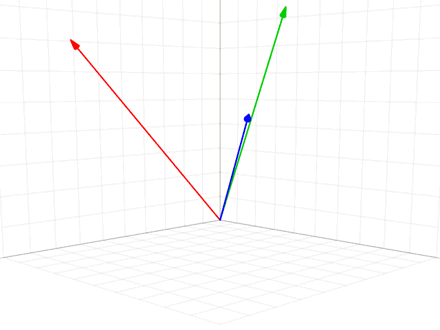
\includegraphics[width=0.45\textwidth]{figure_man/frame_010_delay-2s.png}
  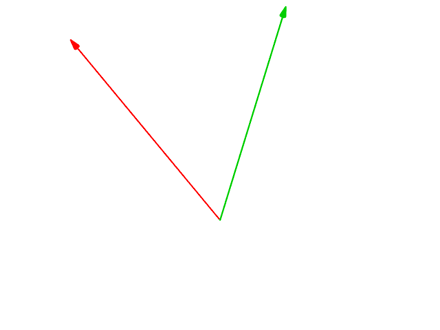
\includegraphics[width=0.45\textwidth]{figure_man/frame_013_delay-1s.png}
\end{figure}
\tiny{\url{https://commons.wikimedia.org/wiki/File:Gram-Schmidt_orthonormalization_process.gif}}

\framebreak

\begin{scriptsize}

\textbf{Given:} Three independent vectors \textcolor{red}{$a_1$}, \textcolor{green}{$a_2$}, \textcolor{blue}{$a_3$} \\
\textbf{Aim:} Vectors of an orthonormal basis \textcolor{red}{$q_1$}, \textcolor{green}{$q_2$}, \textcolor{blue}{$q_3$}

\setbeamercovered{transparent}
\begin{enumerate}
  \item<2-> \textcolor{red}{$a_1$} serves as the first vector of the orthogonal basis (\textcolor{red}{$u_1$}).
  \item \textcolor{green}{$a_2$} is projected onto \textcolor{red}{$u_1$}; projection is substracted from \textcolor{green}{$a_2$}
        to obtain \textcolor{green}{$u_2$}.
  \item<3-> \textcolor{blue}{$a_3$} is projected onto \textcolor{red}{$u_1$} and \textcolor{green}{$u_2$},
        to obtain \textcolor{blue}{$u_3$}.
  \item<4-> \textcolor{red}{$u_1$}, \textcolor{green}{$u_2$} and \textcolor{blue}{$u_3$} are normalized.
\end{enumerate}

\end{scriptsize}

\begin{figure}
  \centering
  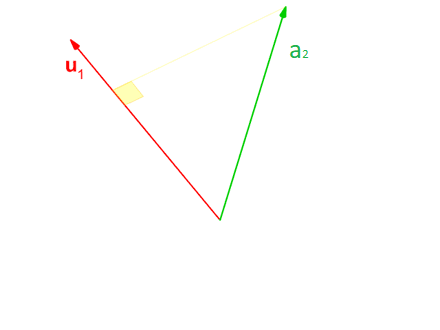
\includegraphics[width=0.33\textwidth]{figure_man/frame_016_delay-3s.png}
  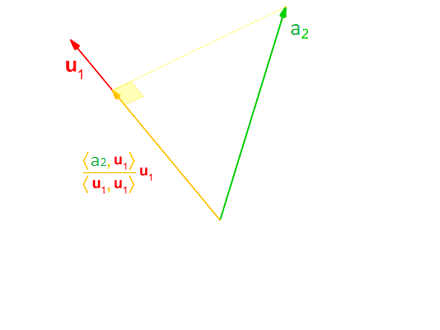
\includegraphics[width=0.33\textwidth]{figure_man/frame_019_delay-3s.png}
  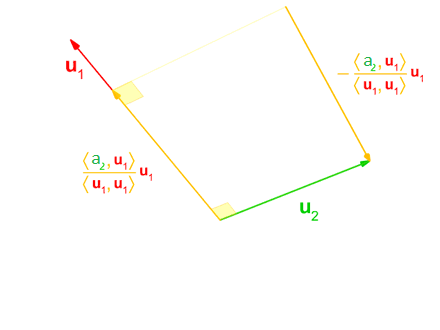
\includegraphics[width=0.33\textwidth]{figure_man/frame_039_delay-4s.png}
\end{figure}
\tiny{\url{https://commons.wikimedia.org/wiki/File:Gram-Schmidt_orthonormalization_process.gif}}

\framebreak

\begin{scriptsize}

\textbf{Given:} Three independent vectors \textcolor{red}{$a_1$}, \textcolor{green}{$a_2$}, \textcolor{blue}{$a_3$} \\
\textbf{Aim:} Vectors of an orthonormal basis \textcolor{red}{$q_1$}, \textcolor{green}{$q_2$}, \textcolor{blue}{$q_3$}

\setbeamercovered{transparent}
\begin{enumerate}
  \item<2-> \textcolor{red}{$a_1$} serves as the first vector of the orthogonal basis (\textcolor{red}{$u_1$}).
  \item<3-> \textcolor{green}{$a_2$} is projected onto \textcolor{red}{$u_1$}; projection is substracted from \textcolor{green}{$a_2$}
        to obtain \textcolor{green}{$u_2$}.
  \item \textcolor{blue}{$a_3$} is projected onto \textcolor{red}{$u_1$} and \textcolor{green}{$u_2$},
        to obtain \textcolor{blue}{$u_3$}.
  \item<4-> \textcolor{red}{$u_1$}, \textcolor{green}{$u_2$} and \textcolor{blue}{$u_3$} are normalized.
\end{enumerate}

\end{scriptsize}

\begin{figure}
  \centering
  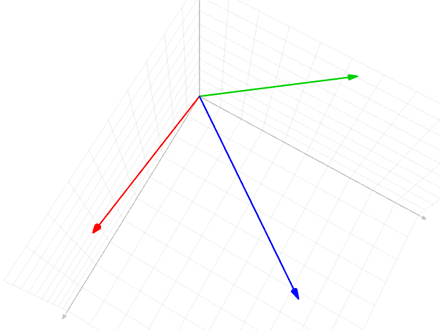
\includegraphics[width=0.45\textwidth]{figure_man/frame_060_delay-2s.png}
  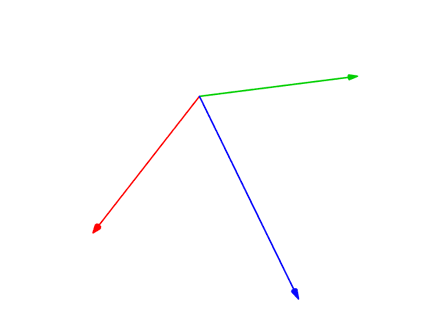
\includegraphics[width=0.45\textwidth]{figure_man/frame_063_delay-1s.png}
\end{figure}
\tiny{\url{https://commons.wikimedia.org/wiki/File:Gram-Schmidt_orthonormalization_process.gif}}

\framebreak

\begin{scriptsize}

\textbf{Given:} Three independent vectors \textcolor{red}{$a_1$}, \textcolor{green}{$a_2$}, \textcolor{blue}{$a_3$} \\
\textbf{Aim:} Vectors of an orthonormal basis \textcolor{red}{$q_1$}, \textcolor{green}{$q_2$}, \textcolor{blue}{$q_3$}

\setbeamercovered{transparent}
\begin{enumerate}
  \item<2-> \textcolor{red}{$a_1$} serves as the first vector of the orthogonal basis (\textcolor{red}{$u_1$}).
  \item<3-> \textcolor{green}{$a_2$} is projected onto \textcolor{red}{$u_1$}; projection is substracted from \textcolor{green}{$a_2$}
        to obtain \textcolor{green}{$u_2$}.
  \item \textcolor{blue}{$a_3$} is projected onto \textcolor{red}{$u_1$} and \textcolor{green}{$u_2$},
        to obtain \textcolor{blue}{$u_3$}.
  \item<4-> \textcolor{red}{$u_1$}, \textcolor{green}{$u_2$} and \textcolor{blue}{$u_3$} are normalized.
\end{enumerate}

\end{scriptsize}

\begin{figure}
  \centering
  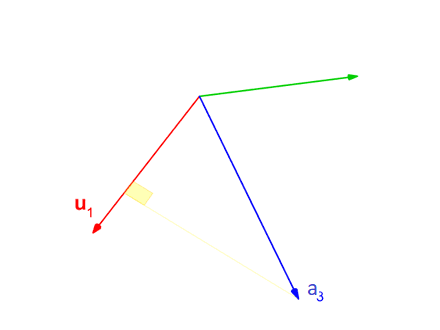
\includegraphics[width=0.33\textwidth]{figure_man/frame_066_delay-3s.png}
  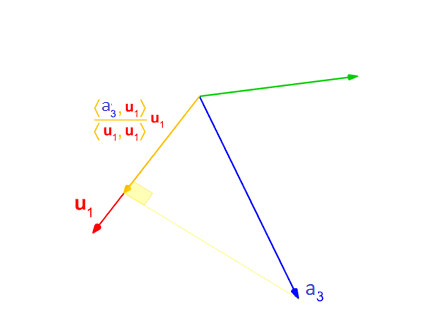
\includegraphics[width=0.33\textwidth]{figure_man/frame_069_delay-3s.png}
  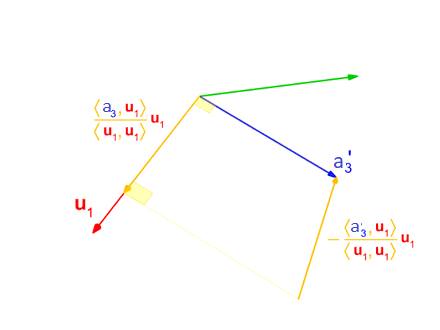
\includegraphics[width=0.33\textwidth]{figure_man/frame_089_delay-4s.png}
\end{figure}
\tiny{\url{https://commons.wikimedia.org/wiki/File:Gram-Schmidt_orthonormalization_process.gif}}

\framebreak

\begin{scriptsize}

\textbf{Given:} Three independent vectors \textcolor{red}{$a_1$}, \textcolor{green}{$a_2$}, \textcolor{blue}{$a_3$} \\
\textbf{Aim:} Vectors of an orthonormal basis \textcolor{red}{$q_1$}, \textcolor{green}{$q_2$}, \textcolor{blue}{$q_3$}

\setbeamercovered{transparent}
\begin{enumerate}
  \item<2-> \textcolor{red}{$a_1$} serves as the first vector of the orthogonal basis (\textcolor{red}{$u_1$}).
  \item<3-> \textcolor{green}{$a_2$} is projected onto \textcolor{red}{$u_1$}; projection is substracted from \textcolor{green}{$a_2$}
        to obtain \textcolor{green}{$u_2$}.
  \item \textcolor{blue}{$a_3$} is projected onto \textcolor{red}{$u_1$} and \textcolor{green}{$u_2$},
        to obtain \textcolor{blue}{$u_3$}.
  \item<4-> \textcolor{red}{$u_1$}, \textcolor{green}{$u_2$} and \textcolor{blue}{$u_3$} are normalized.
\end{enumerate}

\end{scriptsize}

\begin{figure}
  \centering
  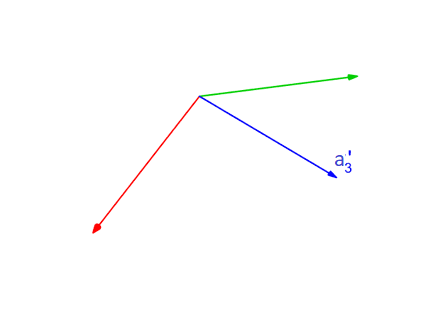
\includegraphics[width=0.45\textwidth]{figure_man/frame_092_delay-1s.png}
  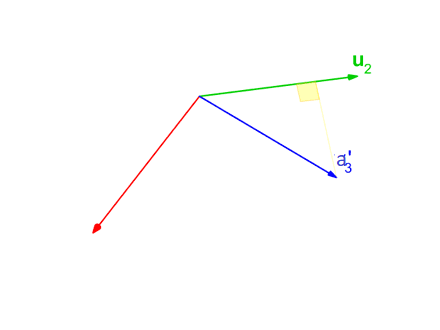
\includegraphics[width=0.45\textwidth]{figure_man/frame_095_delay-3s.png}
\end{figure}
\tiny{\url{https://commons.wikimedia.org/wiki/File:Gram-Schmidt_orthonormalization_process.gif}}

\framebreak

\begin{scriptsize}

\textbf{Given:} Three independent vectors \textcolor{red}{$a_1$}, \textcolor{green}{$a_2$}, \textcolor{blue}{$a_3$} \\
\textbf{Aim:} Vectors of an orthonormal basis \textcolor{red}{$q_1$}, \textcolor{green}{$q_2$}, \textcolor{blue}{$q_3$}

\setbeamercovered{transparent}
\begin{enumerate}
  \item<2-> \textcolor{red}{$a_1$} serves as the first vector of the orthogonal basis (\textcolor{red}{$u_1$}).
  \item<3-> \textcolor{green}{$a_2$} is projected onto \textcolor{red}{$u_1$}; projection is substracted from \textcolor{green}{$a_2$}
        to obtain \textcolor{green}{$u_2$}.
  \item \textcolor{blue}{$a_3$} is projected onto \textcolor{red}{$u_1$} and \textcolor{green}{$u_2$},
        to obtain \textcolor{blue}{$u_3$}.
  \item<4-> \textcolor{red}{$u_1$}, \textcolor{green}{$u_2$} and \textcolor{blue}{$u_3$} are normalized.
\end{enumerate}

\end{scriptsize}

\begin{figure}
  \centering
  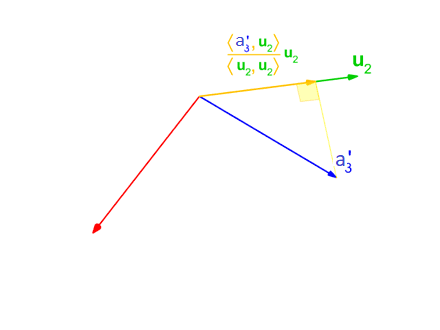
\includegraphics[width=0.45\textwidth]{figure_man/frame_098_delay-3s.png}
  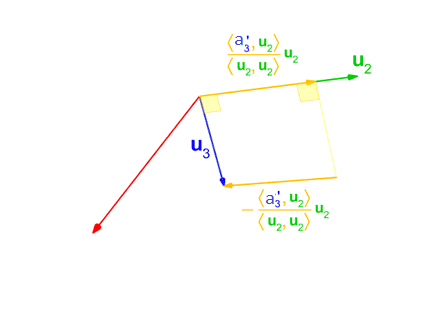
\includegraphics[width=0.45\textwidth]{figure_man/frame_118_delay-4s.png}
\end{figure}
\tiny{\url{https://commons.wikimedia.org/wiki/File:Gram-Schmidt_orthonormalization_process.gif}}

\framebreak

\begin{scriptsize}

\textbf{Given:} Three independent vectors \textcolor{red}{$a_1$}, \textcolor{green}{$a_2$}, \textcolor{blue}{$a_3$} \\
\textbf{Aim:} Vectors of an orthonormal basis \textcolor{red}{$q_1$}, \textcolor{green}{$q_2$}, \textcolor{blue}{$q_3$}

\setbeamercovered{transparent}
\begin{enumerate}
  \item<2-> \textcolor{red}{$a_1$} serves as the first vector of the orthogonal basis (\textcolor{red}{$u_1$}).
  \item<3-> \textcolor{green}{$a_2$} is projected onto \textcolor{red}{$u_1$}; projection is substracted from \textcolor{green}{$a_2$}
        to obtain \textcolor{green}{$u_2$}.
  \item<4-> \textcolor{blue}{$a_3$} is projected onto \textcolor{red}{$u_1$} and \textcolor{green}{$u_2$},
        to obtain \textcolor{blue}{$u_3$}.
  \item \textcolor{red}{$u_1$}, \textcolor{green}{$u_2$} and \textcolor{blue}{$u_3$} are normalized.
\end{enumerate}

\end{scriptsize}

\begin{figure}
  \centering
  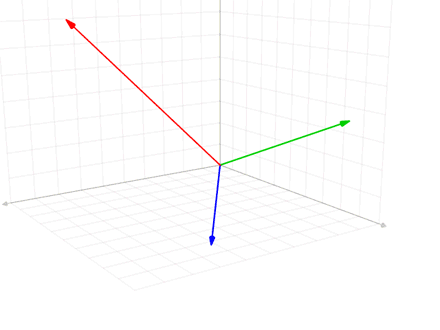
\includegraphics[width=0.45\textwidth]{figure_man/frame_131_delay-2s.png}
  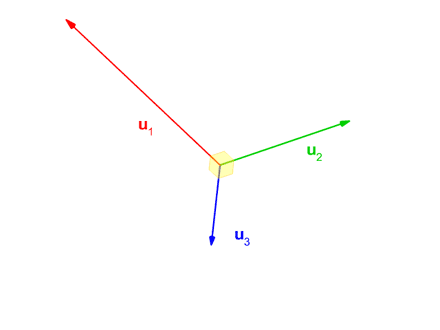
\includegraphics[width=0.45\textwidth]{figure_man/frame_134_delay-3s.png}
\end{figure}
\tiny{\url{https://commons.wikimedia.org/wiki/File:Gram-Schmidt_orthonormalization_process.gif}}

\framebreak

\begin{scriptsize}

\textbf{Given:} Three independent vectors \textcolor{red}{$a_1$}, \textcolor{green}{$a_2$}, \textcolor{blue}{$a_3$} \\
\textbf{Aim:} Vectors of an orthonormal basis \textcolor{red}{$q_1$}, \textcolor{green}{$q_2$}, \textcolor{blue}{$q_3$}

\setbeamercovered{transparent}
\begin{enumerate}
  \item<2-> \textcolor{red}{$a_1$} serves as the first vector of the orthogonal basis (\textcolor{red}{$u_1$}).
  \item<3-> \textcolor{green}{$a_2$} is projected onto \textcolor{red}{$u_1$}; projection is substracted from \textcolor{green}{$a_2$}
        to obtain \textcolor{green}{$u_2$}.
  \item<4-> \textcolor{blue}{$a_3$} is projected onto \textcolor{red}{$u_1$} and \textcolor{green}{$u_2$},
        to obtain \textcolor{blue}{$u_3$}.
  \item \textcolor{red}{$u_1$}, \textcolor{green}{$u_2$} and \textcolor{blue}{$u_3$} are normalized.
\end{enumerate}

\end{scriptsize}

\begin{figure}
  \centering
  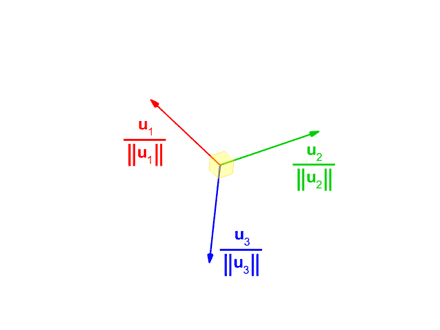
\includegraphics[width=0.45\textwidth]{figure_man/frame_144_delay-3s.png}
  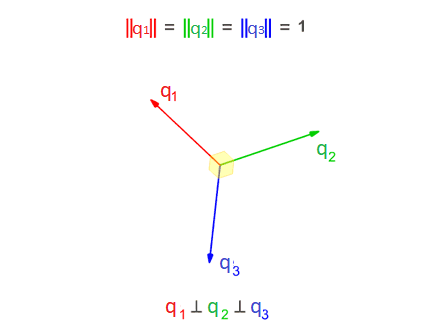
\includegraphics[width=0.45\textwidth]{figure_man/frame_149_delay-8s.png}
\end{figure}
\tiny{\url{https://commons.wikimedia.org/wiki/File:Gram-Schmidt_orthonormalization_process.gif}}

\end{vbframe}

\begin{vbframe}{QR decomposition: Example}

Calculation of $\bm{A} = \bm{Q}\bm{R}$ with $\bm{A}$ given by

\begin{footnotesize}
$$
\Amat = \begin{pmatrix*}[r]
0 & -20 & -14 \\
3 & 27 & -4 \\
4 & 11 & -2 \end{pmatrix*}
$$
\end{footnotesize}

\begin{footnotesize}
$k = 1$:
\vspace*{-0.5cm}
\begin{align*}
  \bm{u}_1 =& \bm{a}_1 = \mat{0 \\ 3 \\ 4} \\
  \bm{q}_1 =& \frac{\bm{u}_1}{\|\bm{u}_1\|} = \frac{\bm{u}_1}{\sqrt{0+9+16}}
           = \frac{1}{5} \mat{0 \\ 3 \\ 4} \\
  r_{11} =& \scp{\bm{q}_1}{\bm{a}_1} = \frac{1}{5} (0^2 + 3^2 + 4^2) = 5 \\
    r_{12} =& \scp{\bm{q}_1}{\bm{a}_2} = \frac{1}{5} (0 \cdot (-20) + 3 \cdot 27 + 4 \cdot 11) = 25 \\
        r_{13} =& \scp{\bm{q}_1}{\bm{a}_3} = \frac{1}{5} (0 \cdot (-14) + 3 \cdot (-4) + 4 \cdot (-2)) = -4
\end{align*}

\framebreak

$k = 2$:

\vspace*{-0.5cm}

\begin{align*}
  \bm{u}_2 =& \bm{a}_2 - \frac{\langle \bm{u}_1, \bm{a}_2 \rangle}{\langle \bm{u}_1, \bm{u}_1 \rangle} \bm{u}_1 \\
           =& \bm{a}_2 - \frac{125}{25} \mat{0 \\ 3 \\ 4} \\
           =& \mat{-20 \\ 12 \\ -9} \\
  \bm{q}_2 =& \frac{\bm{u}_2}{\|\bm{u}_2\|} = \frac{\bm{u}_2}{\sqrt{400+144+81}}
           = \frac{1}{25} \mat{-20 \\ 12 \\ -9} \\
               r_{22} =& \scp{\bm{q}_2}{\bm{a}_2} = \frac{1}{25} ((-20) \cdot (-20) + 12 \cdot 27 + (-9) \cdot 11) = 25 \\
           r_{23} =& \scp{\bm{q}_2}{\bm{a}_3} = \frac{1}{25} ((-20) \cdot (-14) + 12 \cdot (-4) + (-9) \cdot (-2)) = 10
\end{align*}

\framebreak

$k = 3$:

\begin{align*}
  \bm{u}_3 =& \bm{a}_3 - \frac{\langle \bm{u}_1, \bm{a}_3 \rangle}{\langle \bm{u}_1, \bm{u}_1 \rangle} \bm{u}_1
                       - \frac{\langle \bm{u}_2, \bm{a}_3 \rangle}{\langle \bm{u}_2, \bm{u}_2 \rangle} \bm{u}_2 \\
           =& \bm{a}_3 - \frac{-20}{25} \mat{0 \\ 3 \\ 4} - \frac{250}{625} \mat{-20 \\ 12 \\ -9} \\
           =& \mat{-6 \\ -6.4 \\ 4.8} \\
  \bm{q}_3 =& \frac{\bm{u}_3}{\|\bm{u}_3\|} = \frac{1}{25} \mat{-15 \\ -16 \\ 12} \\
  r_{33} =& \scp{\bm{q}_3}{\bm{a}_3} = \frac{1}{25} ((-15) \cdot (-14) + (-16) \cdot (-4) + 12 \cdot (-2)) = 10
\end{align*}
\end{footnotesize}

\framebreak


% \medskip
% $r_{13} \leftarrow \mathbf{q}_1^\top\mathbf{x}_3 = -4$ und $r_{23} \leftarrow \mathbf{q}_2^\top\mathbf{x}_3 = 10$
% $\mathbf{q}_3 \leftarrow \mathbf{x}_3 - r_{13}\mathbf{q}_1 - r_{23}\mathbf{q}_2 = \frac{2}{5}
%   \begin{pmatrix*}[r] -15 \\ -16 \\ 12\end{pmatrix*}$ \\
% $r_{33} \leftarrow \|\mathbf{q}_3\| = 10$ und $\mathbf{q}_3 \leftarrow \frac{\mathbf{q}_3}{r_{33}} =
%   \frac{1}{25} \begin{pmatrix*}[r] -15 \\ -16 \\ 12 \end{pmatrix*}$\\
% \medskip

\framebreak

This results in
$$
\mathbf{Q} = \frac{1}{25} \begin{pmatrix*}[r]
0 & -20 & -15 \\
15 & 12 & -16 \\
20 & -9 & 12 \end{pmatrix*}
\quad \text{ and } \quad \mathbf{R} = \begin{pmatrix*}[r]
5 & 25 & -4 \\
0 & 25 & 10 \\
0 & 0 & 10 \end{pmatrix*}.
$$

\end{vbframe}


\begin{vbframe}{Householder and Givens matrix}

\vspace*{-0.2cm}
\textbf{Problem in practice:}\\
$\mathbf{Q}$ often not really orthogonal when using the above algorithm due to numerical reasons.\\
\vspace*{0.2cm}
Two other methods for QR decomposition\\
\medskip
{\bf Householder matrix:}\\
\medskip
For vector $\mathbf{u}$, matrix $\mathbf{U} = \mathbf{I} - d\mathbf{uu}^\top$ is orthogonal,
if $d = 2/ \mathbf{u}^\top\mathbf{u}$.
Choose $\mathbf{u} = \mathbf{x} + s\mathbf{e}_1$ with $s = \mathbf{x}^\top\mathbf{x}$
$\quad \Rightarrow \quad \mathbf{Ux} = - s\mathbf{e}_1$.\\
\medskip
Successive elimination of column elements yields QR decomposition.\\
\medskip
{\bf Givens matrix:}\\
\medskip
Similar to Householder, but orthogonal transformations that eliminate an element of a column vector each, and change a second vector. \\
\medskip

\begin{footnotesize}
For details see Carl D.\ Meyer \emph{Matrix Analysis and Applied Linear Algebra}.
\end{footnotesize}

\end{vbframe}

\begin{vbframe} {Properties of QR decomposition}

\begin{itemize}
\item Splitting a matrix into an orthogonal matrix $\mathbf{Q}$ and $\mathbf{R}$
% \item $\Amat$ is split into a lower triangle matrix $\mathbf{L}$ and a lower triangle matrix $\mathbf{U}$.
\item Gram-Schmidt process is numerically unstable, but can be extended and numerically stabilized
\item \textbf{Existence:} Decomposition exists for each $n \times n$ matrix and can be extended to general $m \times n, m \ne n$ matrices
\item Runtime behavior: Numerical stable solution of Householder transformation or Givens rotation comes along with higher effort:
\begin{itemize}
\item Decomposition of $n \times n$ matrix using Householder transformation: $\approx \frac{2}{3}n^3$ multiplications
\item Forward and back substitution: $n^2$
\end{itemize}
% $\to$ Gesamtaufwand von $\order(n^3)$
% \item Rechnung für Zerlegung kann auf Speicher der Matrix $\Amat$ durchgeführt werden \\
% $\to$ kein zusätzlicher Speicher nötig
\end{itemize}

\end{vbframe}

\begin{vbframe}{Comparison of methods}

\begin{table}
\centering
\begin{tabular}{c|c|c|c}
Procedure & $\mathbf{A}$ & \# Multiplications & Stability \\
\hline
LU & regular & $\approx \frac{1}{3} n^3$ & yes, by pivoting \\
Cholesky & p.d. & $\approx \frac{1}{6}n^3$ & yes \\
QR (Gram Schmidt) & - & $\approx 2n^3$ & no \\
QR (Householder) & - & $\approx \frac{2}{3}n^3$ & yes \\
\end{tabular}
\end{table}


\end{vbframe}

\begin{vbframe}{QR decomposition for $m \times n$ matrices}

General $m \times n, m \ge n$ matrices can be decomposed as well when using QR decomposition.

$$
\Amat = \bm{QR} = \bm{Q} \begin{bmatrix} \bm{R}_1 \\ \mathbf{0} \end{bmatrix} = \begin{bmatrix} \bm{Q}_1 & \bm{Q}_2 \end{bmatrix} \begin{bmatrix} \bm{R}_1 \\ \mathbf{0} \end{bmatrix} = \bm{Q}_1 \bm{R}_1
$$

$\bm{Q}_1 \in \R^{m \times n}, \bm{Q}_2 \in \R^{m\times(m-n)}$ with orthogonal columns, and $\bm{R} \in \R^{n \times n}$ upper triangular matrix.

\lz

$\bm{Q}_1 \times \bm{R}_1$ is known as a \textbf{reduced} QR decomposition.

\end{vbframe}


\endlecture
\end{document}







